\documentclass[a4paper,12pt]{article}

\usepackage{geometry}
\usepackage{polski}
\usepackage{amsmath}
\usepackage{ragged2e}
\usepackage{graphicx}
\usepackage{xcolor}
\usepackage{siunitx}
\usepackage{multirow}
\usepackage{pdfpages}

\graphicspath{ {./images/} }

\newcommand\crule[3][black]{\textcolor{#1}{\rule{#2}{#3}}}

\geometry{
 a4paper,
 total={170mm,257mm},
 left=20mm,
 top=20mm,
 }

\definecolor{amethyst}{rgb}{0.6, 0.4, 0.8}

\begin{document}
\title{Układy Elektroniczne - Logika kombinacyjna}
\author{Piotr Moszkowicz} 
\date{\today}
\maketitle
\pagenumbering{roman}

\newpage
\begin{justify}
\tableofcontents
\newpage
\pagenumbering{arabic}

\section{Cel i zakres ćwiczenia}

Celem ćwiczenia zapoznanie się z logiką kombinacyjną oraz wykorzystanie jej w celu utworzenia prostych układów WE/WY, które wykonują zadaną funkcję.

\section{Schemat płytki PLD}

\begin{figure}[h!]
\centering
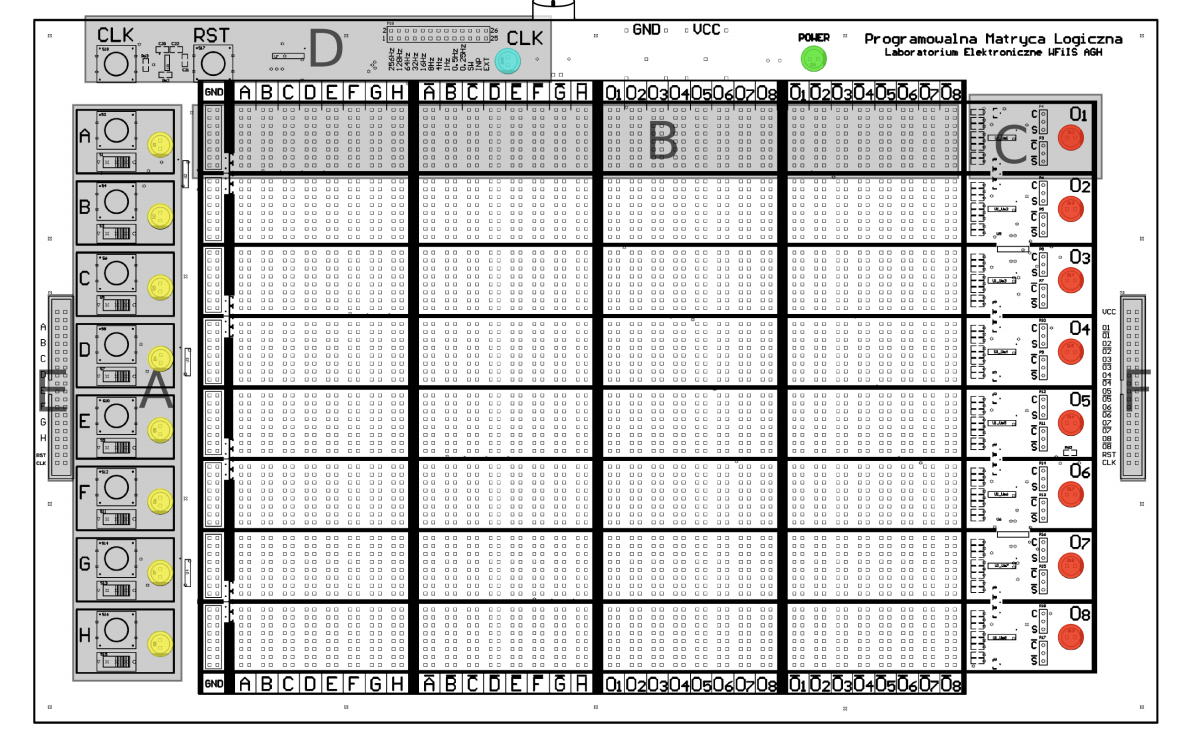
\includegraphics[width=15cm, height=8cm]{pld}
\end{figure}

\section{Pomiary i wyniki}

\subsection{Bramki logiczne wykorzystywane w logice kombinacyjnej}

Każdy układ, który budujemy składa się z bramek logicznych. W logice kombinacyjnej wyróżniamy 7 typów bramek: NOT, AND, NAND, OR, NOR, XOR, XNOR. Istotną informacją jest to, iż z pomocą samych bramek NAND lub samych bramek NOR możemy zbudować dowolną funkcję logiczną (również inne bramki). Z tego powodu te dwie bramki nazywane są \textbf{funkcjonalnie pełnymi}. Poniżej lista wszystkich bramek wraz z ich symbolami, funkcjami logicznymi, tabelami prawd oraz realizacją zworkową na płytce PLD.

\newpage

\subsubsection{Bramka NOT}

\begin{figure}[h!]
\centering
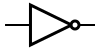
\includegraphics[width=2cm, height=1cm]{NOT}
\end{figure}

Funkcja w algebrze boolowskiej: $\overline{A}$

Tabela prawdy:

\begin{table}[h!]
\begin{center}
\begin{scriptsize}
\begin{tabular}{|c|c|}
\hline
IN & OUT  \\
\hline
A & $\overline{A}$ \\
\hline
0 & 1 \\
1 & 0 \\
\hline
\end{tabular}
\end{scriptsize}
\end{center}
\end{table}

Realizacja zworkowa:

\begin{figure}[h!]
\centering
\includegraphics[width=18cm, height=3cm]{Z_NOT}
\end{figure}

\subsubsection{Bramka AND}

\begin{figure}[h!]
\centering
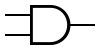
\includegraphics[width=2cm, height=1cm]{AND}
\end{figure}

Funkcja w algebrze boolowskiej: $A \cdot B$

Tabela prawdy:

\begin{table}[h!]
\begin{center}
\begin{scriptsize}
\begin{tabular}{|c|c|c|}
\hline
\multicolumn{2}{|c}{IN} & OUT  \\
\hline
A & B & $A \cdot B$ \\
\hline
0 & 0 & 0 \\
0 & 1 & 0 \\
1 & 0 & 0 \\
1 & 1 & 1 \\
\hline
\end{tabular}
\end{scriptsize}
\end{center}
\end{table}

Realizacja zworkowa:

\begin{figure}[h!]
\centering
\includegraphics[width=18cm, height=3cm]{Z_AND}
\end{figure}

\newpage

\subsubsection{Bramka NAND}

\begin{figure}[h!]
\centering
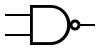
\includegraphics[width=2cm, height=1cm]{NAND}
\end{figure}

Funkcja w algebrze boolowskiej: $\overline{A \cdot B}$

Tabela prawdy:

\begin{table}[h!]
\begin{center}
\begin{scriptsize}
\begin{tabular}{|c|c|c|}
\hline
\multicolumn{2}{|c}{IN} & OUT  \\
\hline
A & B & $\overline{A \cdot B}$ \\
\hline
0 & 0 & 1 \\
0 & 1 & 1 \\
1 & 0 & 1 \\
1 & 1 & 0 \\
\hline
\end{tabular}
\end{scriptsize}
\end{center}
\end{table}

Realizacja zworkowa:

\begin{figure}[h!]
\centering
\includegraphics[width=18cm, height=3cm]{Z_NAND}
\end{figure}

\subsubsection{Bramka OR}

\begin{figure}[h!]
\centering
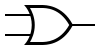
\includegraphics[width=2cm, height=1cm]{OR}
\end{figure}

Funkcja w algebrze boolowskiej: $A + B$

Tabela prawdy:

\begin{table}[h!]
\begin{center}
\begin{scriptsize}
\begin{tabular}{|c|c|c|}
\hline
\multicolumn{2}{|c}{IN} & OUT  \\
\hline
A & B & $A + B$ \\
\hline
0 & 0 & 0 \\
0 & 1 & 1 \\
1 & 0 & 1 \\
1 & 1 & 1 \\
\hline
\end{tabular}
\end{scriptsize}
\end{center}
\end{table}

Realizacja zworkowa:

\begin{figure}[h!]
\centering
\includegraphics[width=18cm, height=3cm]{Z_OR}
\end{figure}

\newpage

\subsubsection{Bramka NOR}

\begin{figure}[h!]
\centering
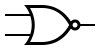
\includegraphics[width=2cm, height=1cm]{NOR}
\end{figure}

Funkcja w algebrze boolowskiej: $\overline{A + B}$

Tabela prawdy:

\begin{table}[h!]
\begin{center}
\begin{scriptsize}
\begin{tabular}{|c|c|c|}
\hline
\multicolumn{2}{|c}{IN} & OUT  \\
\hline
A & B & $\overline{A + B}$ \\
\hline
0 & 0 & 1 \\
0 & 1 & 0 \\
1 & 0 & 0 \\
1 & 1 & 0 \\
\hline
\end{tabular}
\end{scriptsize}
\end{center}
\end{table}

Realizacja zworkowa:

\begin{figure}[h!]
\centering
\includegraphics[width=18cm, height=3cm]{Z_NOR}
\end{figure}

\subsubsection{Bramka XOR}

\begin{figure}[h!]
\centering
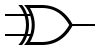
\includegraphics[width=2cm, height=1cm]{XOR}
\end{figure}

Funkcja w algebrze boolowskiej: $A \oplus B$

Tabela prawdy:

\begin{table}[h!]
\begin{center}
\begin{scriptsize}
\begin{tabular}{|c|c|c|}
\hline
\multicolumn{2}{|c}{IN} & OUT  \\
\hline
A & B & $A \oplus B$ \\
\hline
0 & 0 & 0 \\
0 & 1 & 1 \\
1 & 0 & 1 \\
1 & 1 & 0 \\
\hline
\end{tabular}
\end{scriptsize}
\end{center}
\end{table}

Realizacja zworkowa:

\begin{figure}[h!]
\centering
\includegraphics[width=18cm, height=3cm]{Z_XOR}
\end{figure}

\newpage

\subsubsection{Bramka XNOR}

\begin{figure}[h!]
\centering
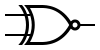
\includegraphics[width=2cm, height=1cm]{XNOR}
\end{figure}

Funkcja w algebrze boolowskiej: $\overline{A \oplus B}$

Tabela prawdy:

\begin{table}[h!]
\begin{center}
\begin{scriptsize}
\begin{tabular}{|c|c|c|}
\hline
\multicolumn{2}{|c}{IN} & OUT  \\
\hline
A & B & $\overline{A \oplus B}$ \\
\hline
0 & 0 & 1 \\
0 & 1 & 0 \\
1 & 0 & 0 \\
1 & 1 & 1 \\
\hline
\end{tabular}
\end{scriptsize}
\end{center}
\end{table}

Realizacja zworkowa:

\begin{figure}[h!]
\centering
\includegraphics[width=18cm, height=3cm]{Z_XNOR}
\end{figure}

\subsection{Czar propagacji sygnału przez bramkę XOR}

Czas propagacji sygnału wynosi 359 ns.

\begin{figure}[h!]
\centering
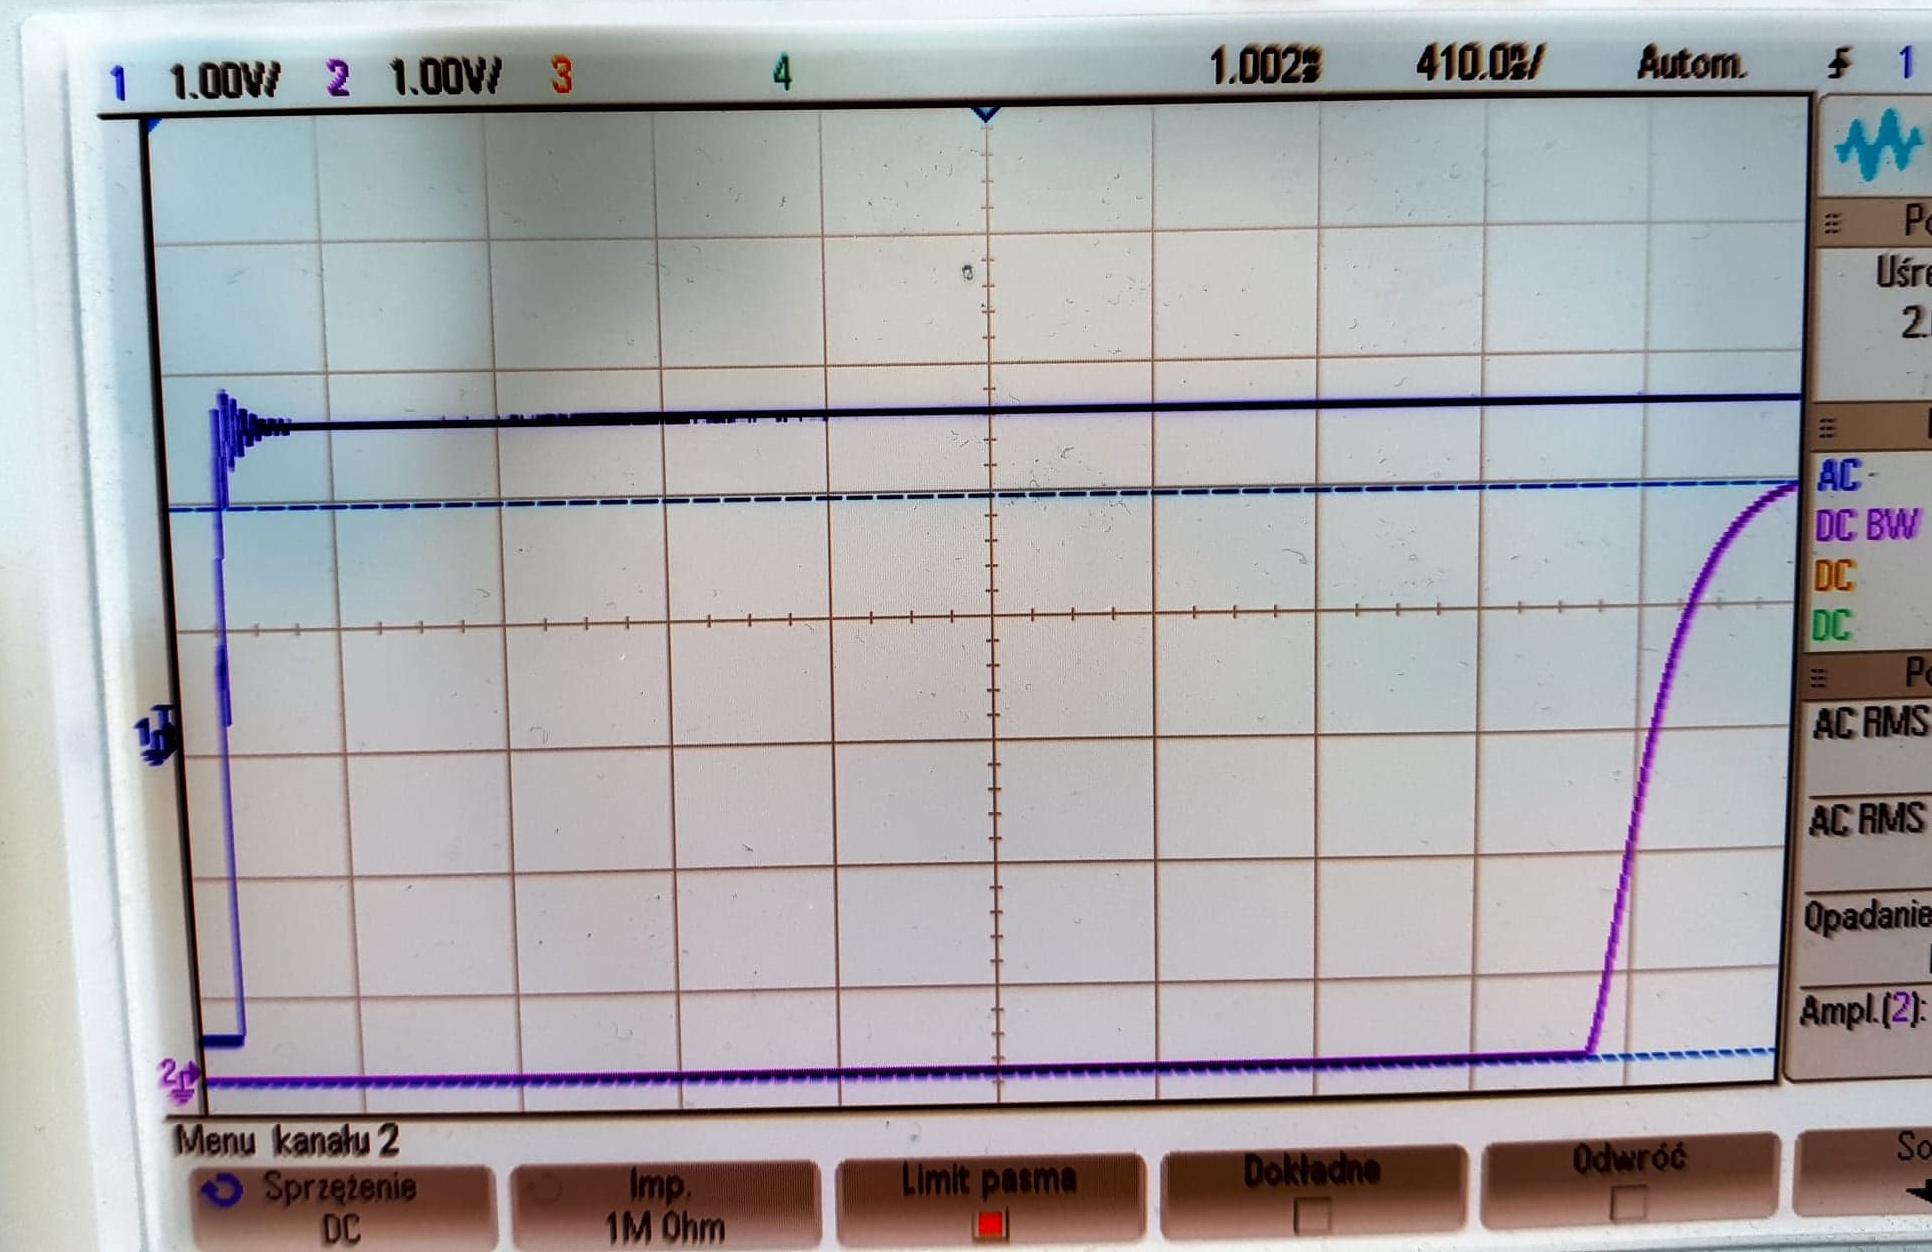
\includegraphics[width=15cm, height=9cm]{narastanie}
\caption{Przebieg narastania sygnału}
\begin{tabular}{cl}
\crule[blue]{1cm}{0.4cm}  & Generator \\
\crule[amethyst]{1cm}{0.4cm}   & Sygnał po przejściu przez bramkę XOR  \\
\end{tabular}
\end{figure}

\newpage

Czas narastania sygnału wynosi 345 ns.

\begin{figure}[h!]
\centering
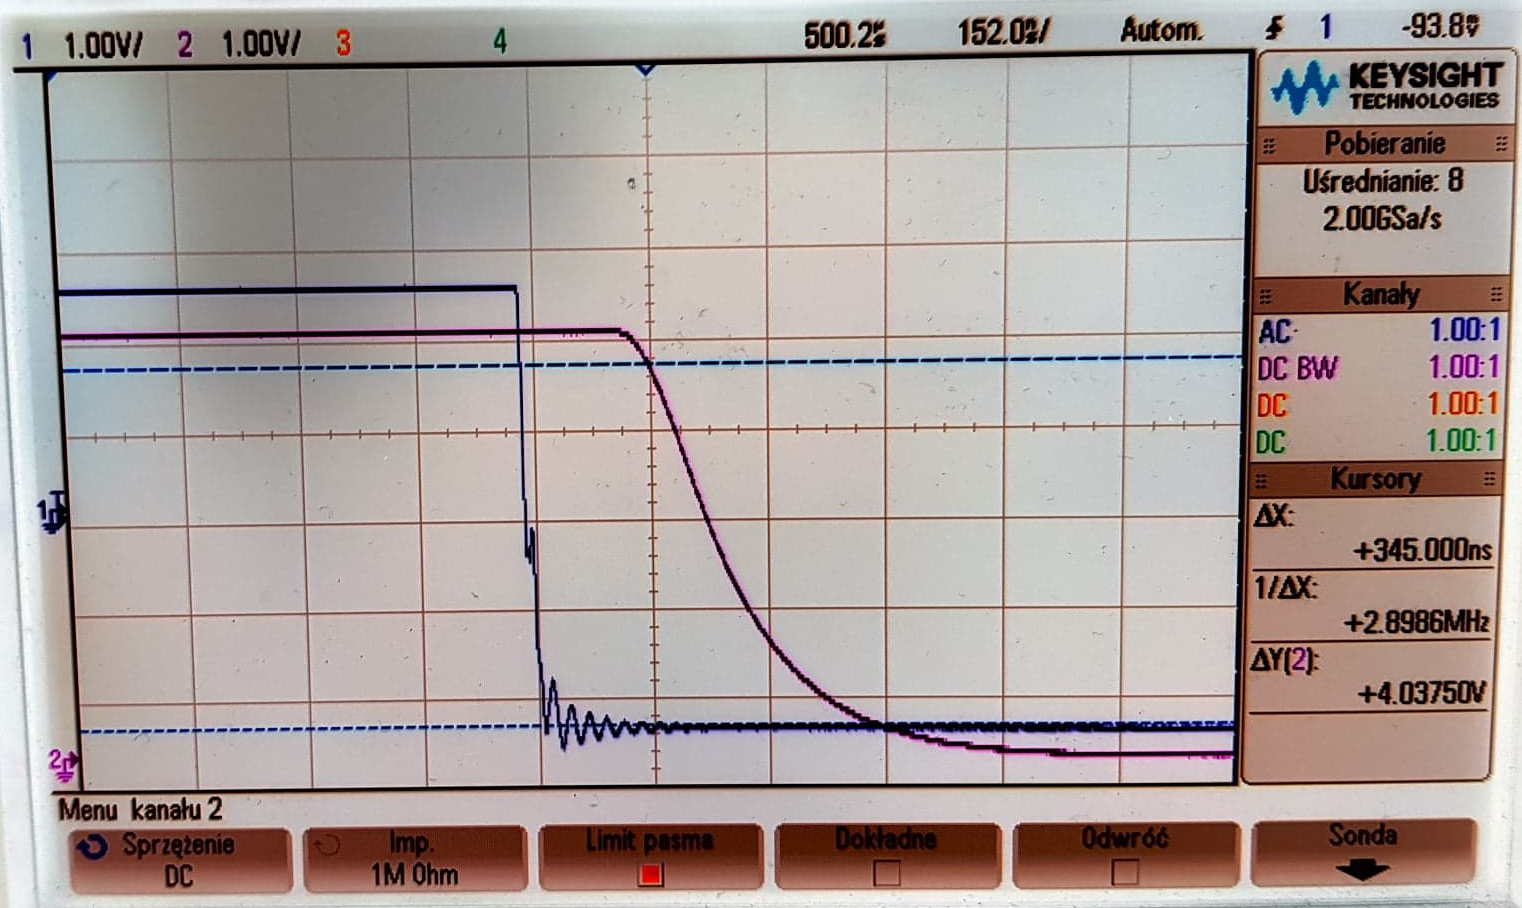
\includegraphics[width=15cm, height=9cm]{opadanie}
\caption{Przebieg odadania sygnału}
\begin{tabular}{cl}
\crule[blue]{1cm}{0.4cm}  & Generator \\
\crule[amethyst]{1cm}{0.4cm}   & Sygnał po przejściu przez bramkę XOR  \\
\end{tabular}
\end{figure}

Czas opadania sygnału wynosi 262 ns.

\subsection{Dekoder kodu binarnego na wyświetlacz 7-segmentowy}

Kolejny zadaniem było skonstruowanie konwertera kodu binarnego na wyświetlacz 7-segmentowy. Moim zdaniem było utworzyć dekoder, który dla liczb 0-9 w kodzie binarnym wyświetla liczby 0-9, a dla kodów od A-F wyświetla "od tyłu" (tj. A - 1010 => wyświetl F). Poniżej widać wszystkich wzory funkcji oraz tabele Karnaugha dla każdej funkcji segmentu (od $O_{1}$ do $O_{7}$). Każda funkcja odpowiada za jedną linię (segment) wyświetlacza. 

\newpage

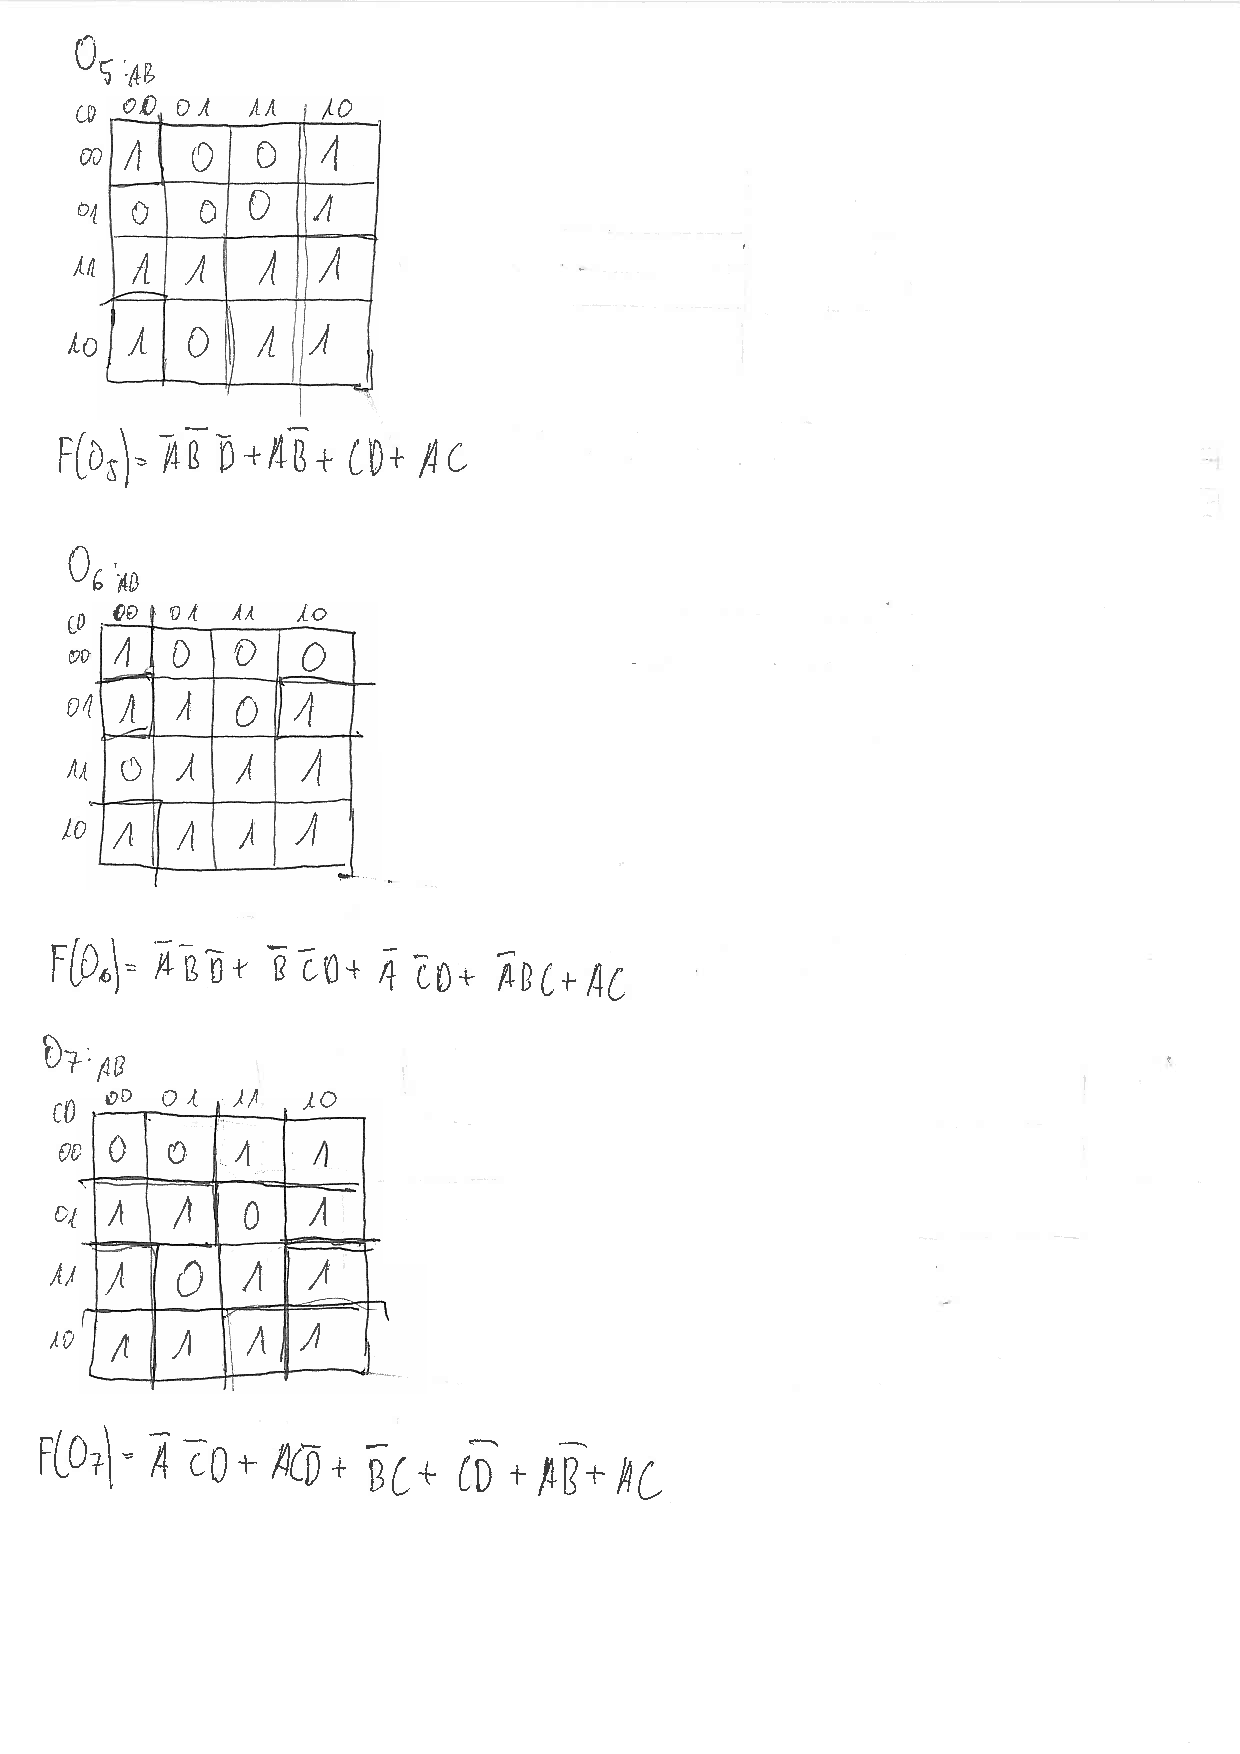
\includepdf[page={2}]{kar}

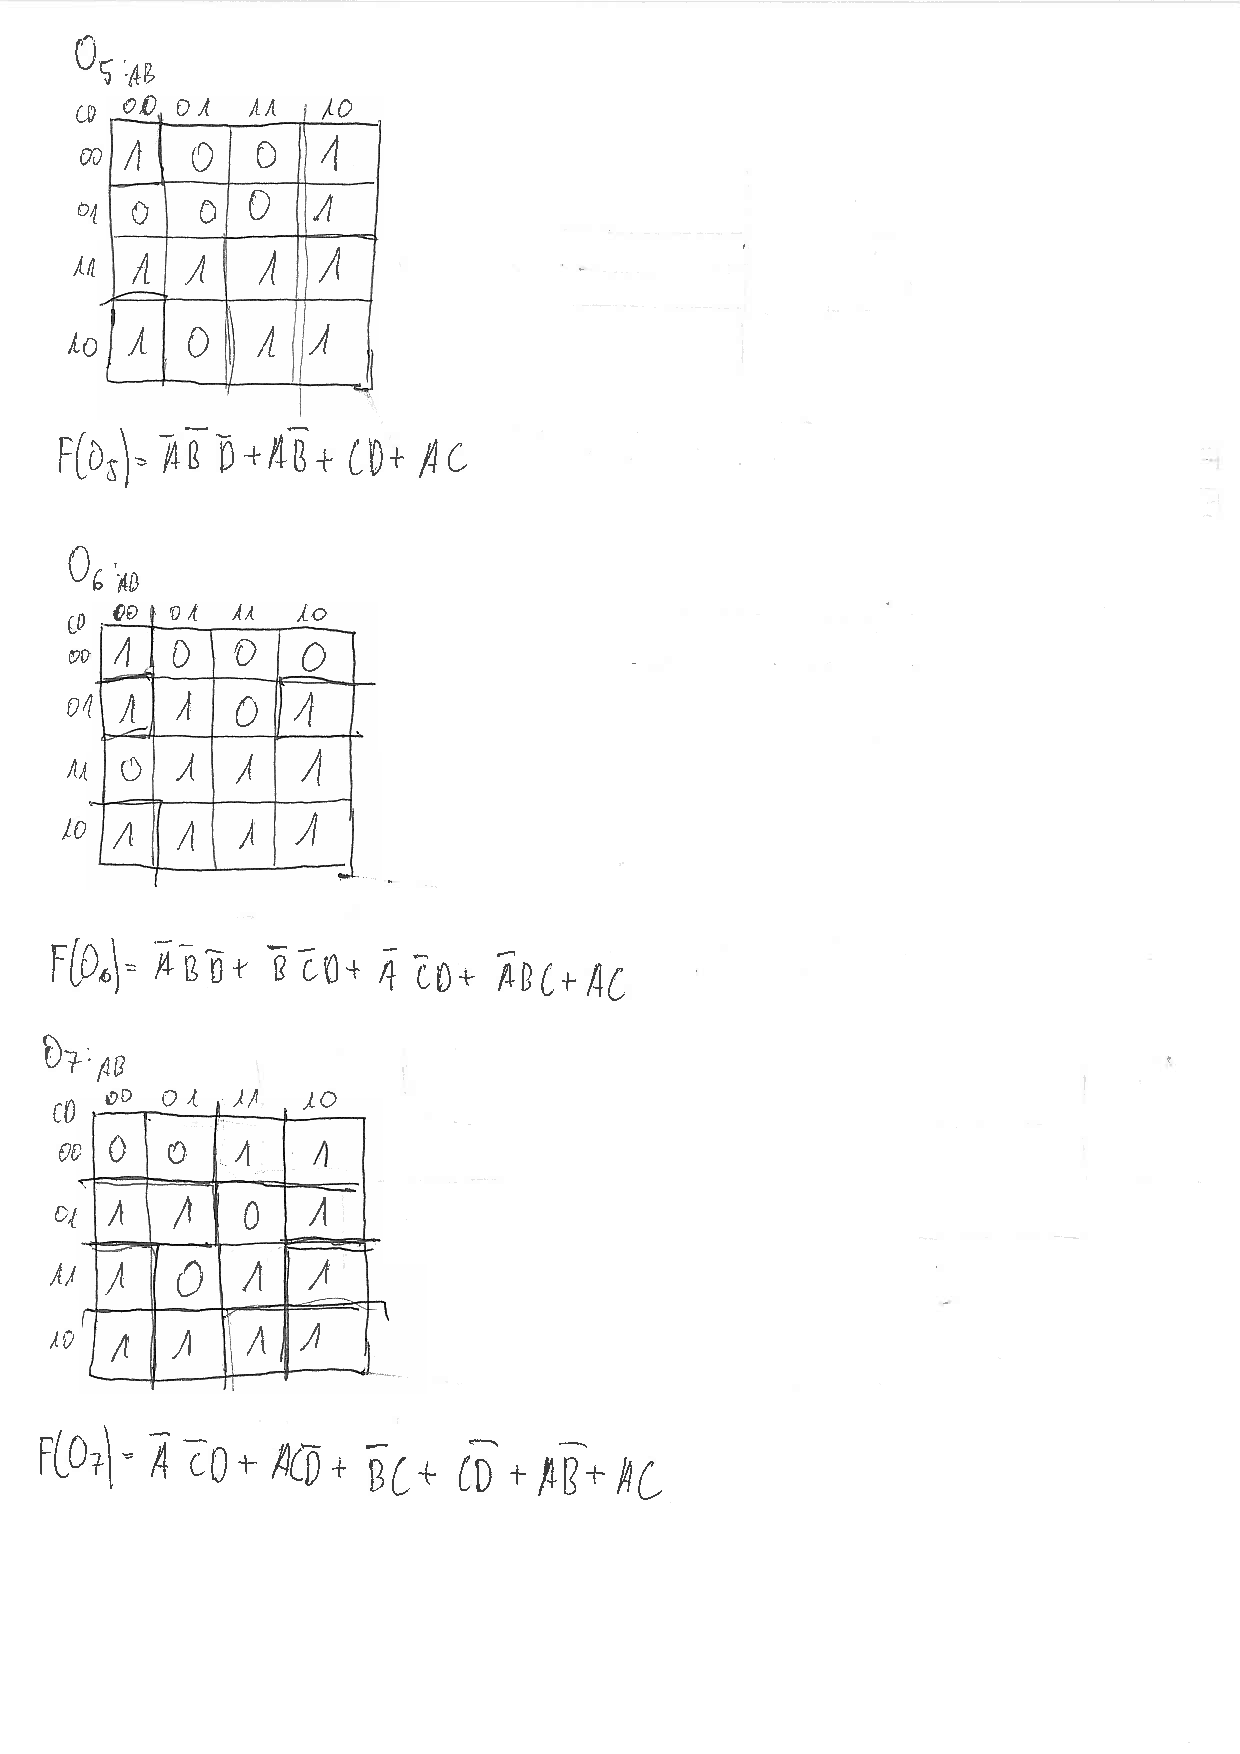
\includepdf[page={1}]{kar}

\newpage

Na poniższym schemacie natomiast można zaobserwować gotową implementację tychże funkcji w postaci zworkowej na matrycy PLD.

\begin{figure}[h!]
\centering
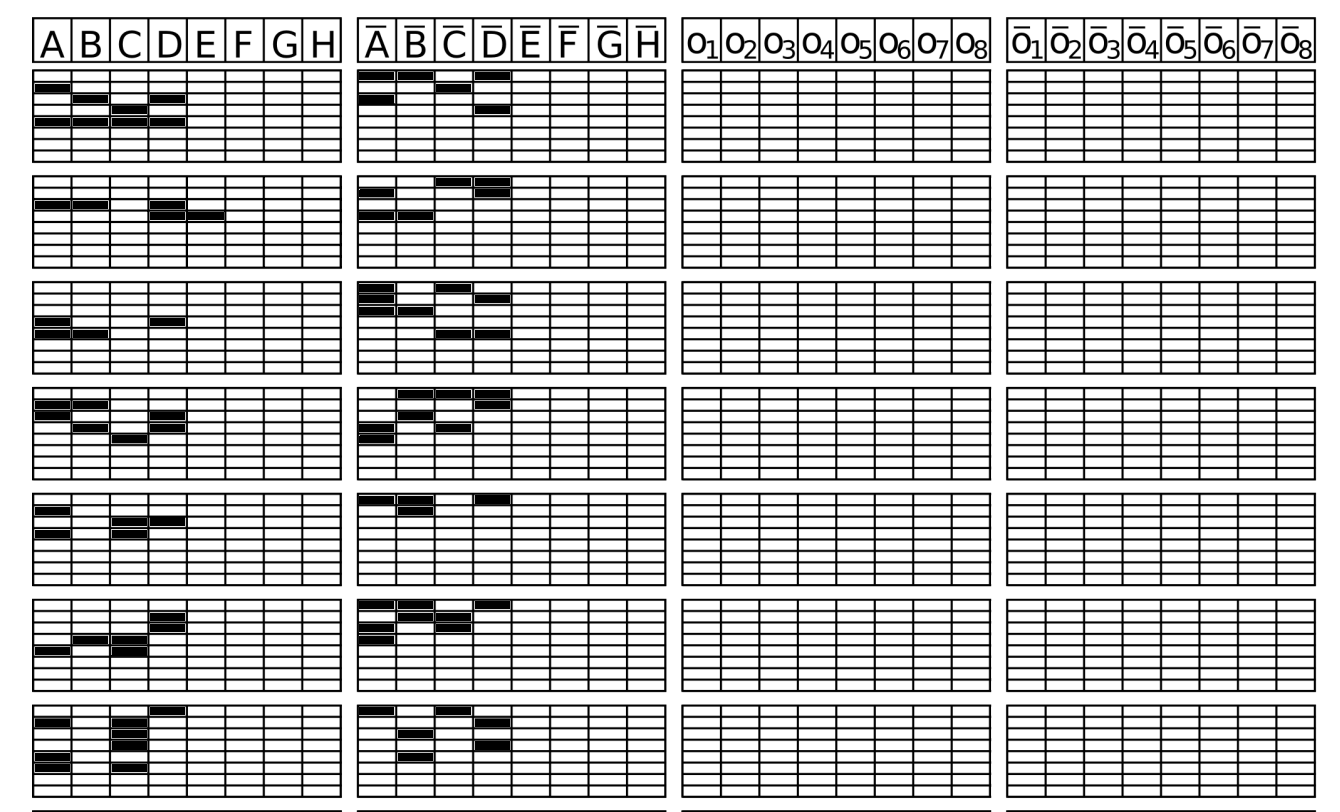
\includegraphics[width=18cm, height=10cm]{Z_DEKODER}
\end{figure}

\end{justify}
\end{document}